\chapter{Objects}
\label{Chp:Objects}

The following \emph{algebraic objects} (operators, monoids, and semirings) are presented in increasing generality.
The ``algebra generality rule'' of GraphBLAS states that a more general object can always be passed to
any method which requires a less general object. The restriction rules are explained in the respective sections of those objects.

Once algebraic objects (operators, monoids and semirings) are described, we introduce \emph{collections} (vectors, matrices and masks) that algebraic objects operate on. Finally, we introduce \emph{descriptors}, which are a simple way to do modify how algebraic objects operate on collections. More concretely, descriptors can be used (among other things) to perform multiplication with transpose of matrix without the user having to manually transpose the collection. A complete list of what descriptors are capable of can be found in the section.

\section{Operators}

A GraphBLAS \emph{binary operators} $F_b = \langle D_1, D_2, D_3, \odot \rangle$
is defined by three domains, $D_1$, $D_2$, $D_3$, and an operation
$\odot: D_1 \times D_2 \rightarrow D_3$.  For a given GraphBLAS operators
$F_b=\langle D_1, D_2, D_3,\odot \rangle$ we define $\bold{D}_1(F_b) = D_1$,
$\bold{D}_2(F_b) = D_2$, $\bold{D}_3(F_b) = D_3$, and $\bold{\bigodot}(F_b)
= \odot$.  Note that $\odot$ could be used in place of either $\oplus$ or $\otimes$.

A GraphBLAS \emph{unary operators} $F_u = \langle D_1, D_2, f\rangle$
is defined by two domains, $D_1$, $D_2$, and an operation
$f: D_1 \rightarrow D_2$.  For a given GraphBLAS operators
$F_u=\langle D_1, D_2, f \rangle$ we define $\bold{D}_1(F_u) = D_1$,
$\bold{D}_2(F_u) = D_2$, and $\bold{f}(F)
= f$.

\begin{table}
	\hrule
	\begin{center}
		\caption{Properties and recipes for building GraphBLAS algebraic objects: Unary Operator, Binary Operator, Monoid and Semiring (composed of operations Add and Times).\newline
			\hspace{\textwidth}Note 1: Output domain of Semiring Times must be same as domain of Semiring Add. This ensures 3 domains in total for Semiring rather than 4.}
		\label{Tab:Operator}
		
		\vspace{1\baselineskip}
		(a) Properties of algebraic objects.
		\vspace{1\baselineskip}
		
		\begin{tabular}{l|l|l|l}
			Object & Must Be Associative & Identity Must Exist & Number of Domains  \\
                        \hline
			Unary Operator & no & no & 2 \\
			Binary Operator & no & no & 3  \\
			Monoid & yes & yes & 1  \\
			Semiring Add & yes & yes  & 1  \\
			Semiring Times & no & no & 3  (Note 1) \\
		\end{tabular}
		
		\vspace{1\baselineskip}
		(b) Recipes for algebraic objects.
		\vspace{1\baselineskip}
		
		\begin{tabular}{l|l|l}
			Object          & Recipe                & Number of Domains  \\ 
                        \hline
			Unary Operator  & Function Pointer      & 2 \\				
			Binary Operator & Function Pointer      & 3  \\	
			Monoid          & Associative Binary Operator with Identity & 1  \\
			Semiring        & Associative Binary Operator with Identity $+$ &3 \\
                                        & Binary Operator &  \\
                        
		\end{tabular}
		
	\end{center}
	\hrule
\end{table}

\section{Monoids}

A GraphBLAS \emph{generalized monoid} (or \emph{monoid} for short) $M =
\langle D_1,\odot,0 \rangle$ is defined by a single domain $D_1$, an 
\emph{associative}\footnote{It is expected that implementations 
will utilize IEEE-754 floating point arithmetic which is not 
strictly associative.} 
operation $\odot: D_1 \times D_1 \rightarrow D_1$,
and an identity element $0 \in D_1$.  For a given GraphBLAS monoid $M=\langle
D_1,\odot,0 \rangle$ we define $\bold{D}_1(M) = D_1$, $\bold{\bigodot}(M) =
\odot$ and $\bold{0}(M) = 0$.  A GraphBLAS monoid is equivalent to 
the conventional \emph{monoid} algebraic structure.

Let $F = \langle D_1,D_1,D_1,\odot \rangle$ be a GraphBLAS binary operator
with element $0 \in D_1$.  Then $M = \langle F,0 \rangle = \langle
D_1,\odot,0 \rangle$ is a GraphBLAS monoid.

\section{Semirings}

A GraphBLAS \emph{semiring} (or \emph{semiring} for short)
$S=\langle D_1,D_2,D_3,\oplus,\otimes,0 \rangle$ is defined by
three domains $D_1$, $D_2$ and $D_3$, an \emph{associative}\footnote{It 
is expected that implementations will utilize IEEE-754 floating 
point arithmetic which is not strictly associative.} 
additive operation $\oplus : D_3 \times D_3 \rightarrow D_3$, 
a multiplicative operation $\otimes : D_1 \times D_2 \rightarrow
D_3$, and an element $0 \in D_3$.
For a given GraphBLAS semiring $S=\langle D_1,
D_2, D_3,\oplus,\otimes,0 \rangle$ we define $\bold{D}_1(S) = D_1$,
$\bold{D}_2(S) = D_2$, $\bold{D}_3(S) = D_3$, $\bold{\bigoplus}(S) =
\oplus$, $\bold{\bigotimes}(S) = \otimes$, and $\zero(S) = 0$. 

Let $F = \langle D_1,D_2,D_3,\otimes \rangle$ be an operator
and let $A = \langle D_3,\oplus,0 \rangle$ be a monoid,
then $S= \langle A,F \rangle = \langle D_1,D_2,D_3,\oplus,\otimes,0 \rangle$
is a semiring.

Note: There must be one GraphBLAS monoid in every semiring which 
serves as the semiring's additive operator and  
specifies the same domain for its inputs and output parameters. 

A UML diagram of the conceptual hierarchy of object classes in GraphBLAS
algebra (binary operators, monoids and semirings) is shown in 
Figure~\ref{Fig:AlgebraHierarchy}.

\begin{figure}[htb]
    \hrule
    \begin{center}
        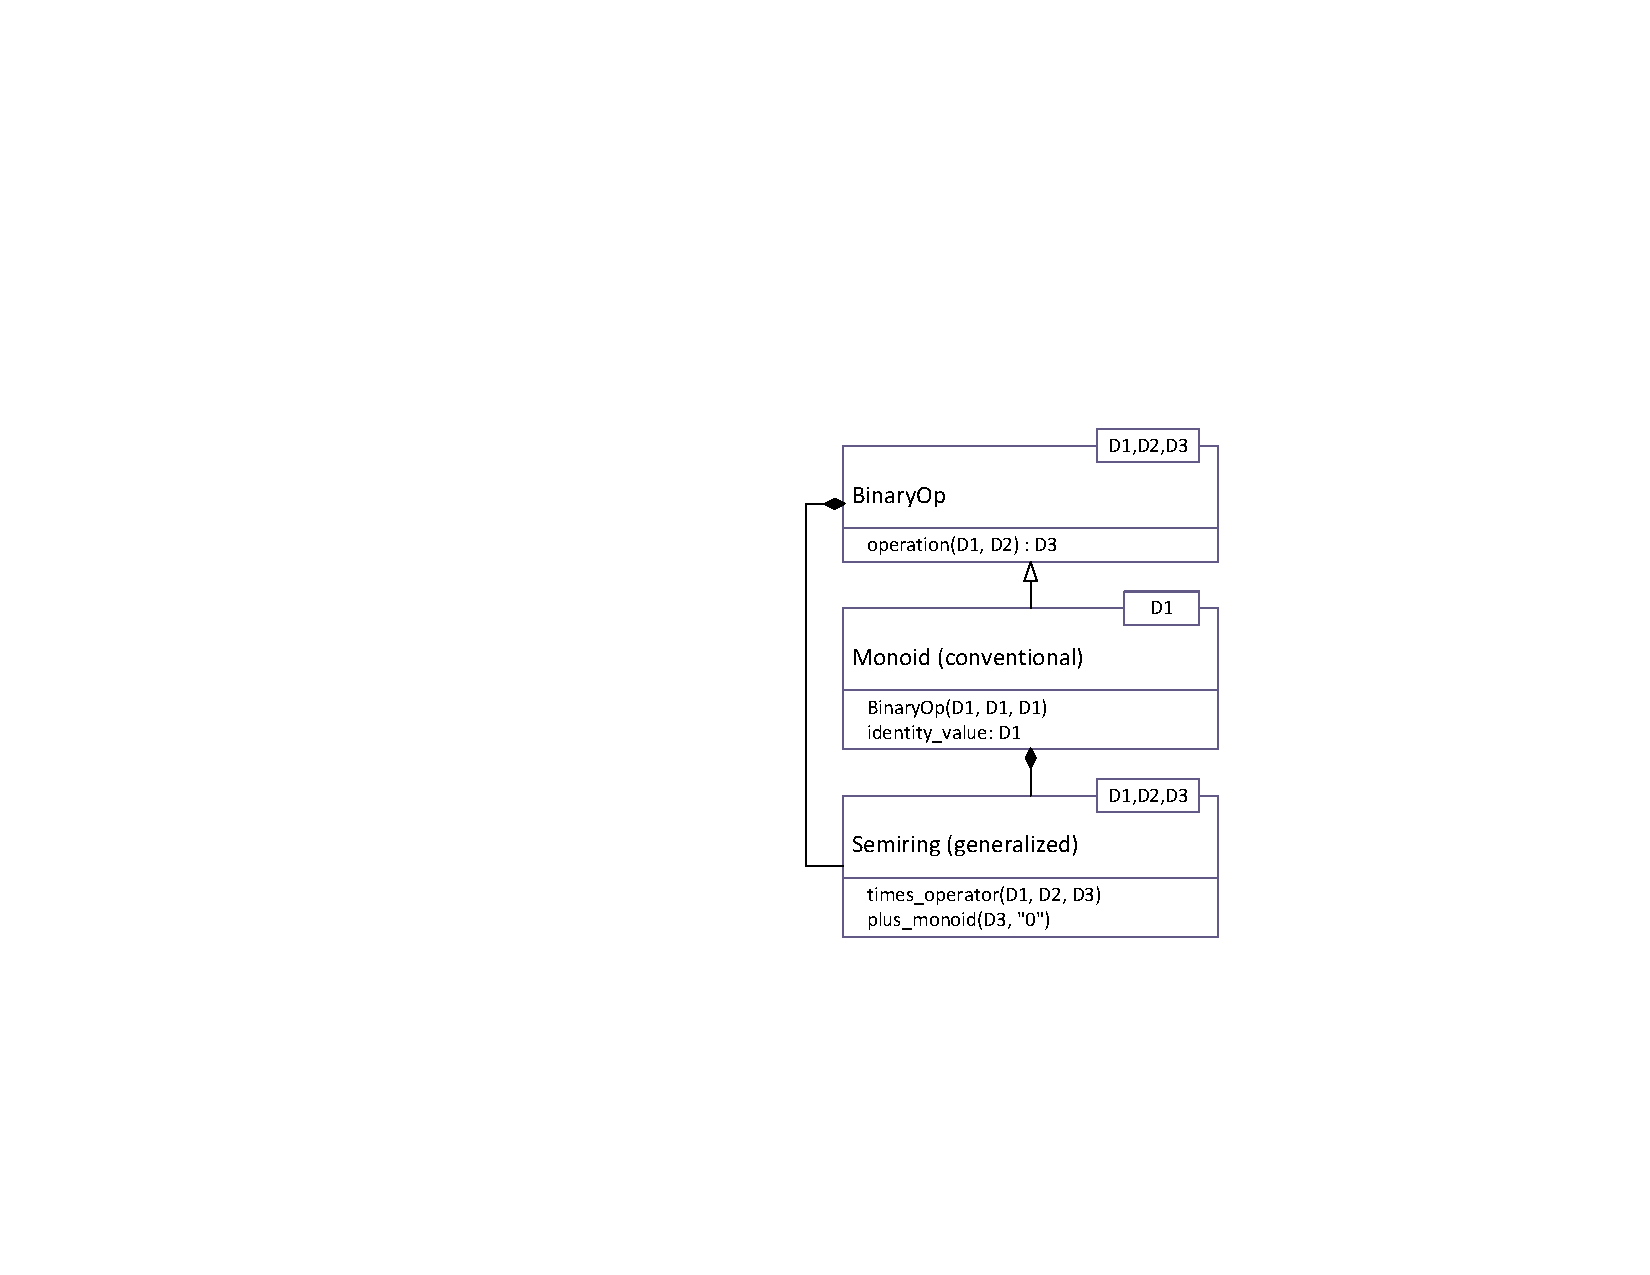
\includegraphics[width=1.0\linewidth,trim=3in 2in 0.5in 2in]{Algebra_Hierarchy_v2.pdf}
    \end{center}
    \caption{Hierarchy of algebraic object classes in GraphBLAS. GraphBLAS semirings consist of a conventional monoid with one domain for the 'add' function, and a binary operator with three domains for the 'multiply' function.}
    \label{Fig:AlgebraHierarchy}
    \hrule
\end{figure}

\begin{table}
    \hrule
    \begin{center}
        \caption{Proposed operator input for relevant GraphBLAS operations. 
        The semiring add and times are shown if applicable.}
        \label{Tab:OperatorInputType}
        \begin{tabular}{l|l}
        Operation           & Operator Input  \\ \hline
        {\sf mxm, mxv, vxm} & Semiring \\ \hline
        {\sf eWiseAdd}      & Binary Operator   \\
                            & Monoid           \\
                            & Semiring          \\ \hline
        {\sf eWiseMult}     & Binary Operator   \\
                            & Monoid          \\
                            & Semiring         \\ \hline
  {\sf reduce} (to vector)  & Binary Operator            \\ 
                            & Monoid           \\ \hline
  {\sf reduce} (to scalar)  & Monoid           \\ \hline
        {\sf apply}         & Unary Operator   \\ \hline
  {\sf buildMatrix} (dups)  & Binary Operator   \\
                            & Monoid           \\ \hline
{\sf accum} param, any op   & Binary Operator  \\
                            & Monoid            \\ 
        \end{tabular}
    \end{center}
    \hrule
\end{table}

\section{Vectors}
\label{Sec:Vectors}

A vector $\vector{v} = \langle D, N, \{ (i,v_i) \} \rangle$ is defined by
a domain $D$, a size $N>0$ and a set of tuples $(i,v_i)$ where $0 \leq
i < N$ and $v_i \in D$. A particular value of $i$ can only appear at
most once in $\vector{v}$. We define $\bold{size}(\vector{v}) = N$ and
$\bold{L}(\vector{v}) = \{ (i,v_i) \}$. The set $\bold{L}(\vector{v})$ is
called the \emph{content} of vector $\vector{v}$. We also define the set
$\vector{ind(\vector{v})} = \{ i : (i,v_i) \in \bold{L}(\vector{v}) \}$
(called the \emph{structure} of $\vector{v}$), and $\bold{D}(\vector{v})
= D$. For a vector $\vector{v}$, $\vector{v}(i)$ is a reference to $v_i$
if $(i,v_i) \in \bold{L}(\vector{v})$ and is undefined otherwise.

\section{Matrices}
\label{Sec:Matrices}

A matrix $\matrix{A} = \langle D, M, N, \{ (i,j,A_{ij}) \} \rangle$ is
defined by a domain $D$, its number of rows $M>0$, its number of columns
$N>0$ and a set of tuples $(i,j,A_{ij})$ where $0 \leq i < M$, $0 \leq
j < N$, and $A_{ij} \in D$. A particular pair of values $i,j$ can only
appear at most once in $\matrix{A}$. We define $\bold{ncols}(\matrix{A})
= N$,  $\bold{nrows}(\matrix{A}) = M$ and $\bold{L}(\matrix{A}) =
\{ (i,j,A_{ij}) \}$.  The set $\bold{L}(\matrix{A})$ is called the
\emph{content} of matrix $\matrix{A}$.  We also define the sets
$\vector{indrow(\matrix{A})} = \{ i : \exists (i,j,A_{ij}) \in
\matrix{A} \}$ and $\vector{indcol(\matrix{A})} = \{ j : \exists
(i,j,A_{ij}) \in \matrix{A} \}$.  (These are the sets of nonempty
rows and columns of $\matrix{A}$, respectively.)  The \emph{structure}
of matrix $\matrix{A}$ is the set $\bold{ind}(\matrix{A}) = \{ (i,j) :
(i,j,A_{ij}) \in \bold{L}(\matrix{A}) \}$, and $\bold{D}(\matrix{A}) = D$.
For a matrix $\matrix{A}$, $\matrix{A}(i,j)$ is a reference to $A_{ij}$
if $(i,j,A_{ij}) \in \bold{L}(\matrix{A})$ and is undefined otherwise.

If $\matrix{A}$ is a matrix and $0 \leq j < N$, then $\matrix{A}(:,j)
= \langle D, M, \{(i,A_{ij}) : (i,j,A_{ij}) \in \bold{L}(\matrix{A})
\} \rangle$ is a vector called the $j$-th \emph{column}
of $\matrix{A}$. Correspondingly, if $\matrix{A}$ is a matrix and
$0 \leq i < M$, then $\matrix{A}(i,:) = \langle D, N, \{(j,A_{ij}) :
(i,j,A_{ij}) \in \bold{L}(\matrix{A}) \} \rangle$ is a vector called
the $i$-th \emph{row} of $\matrix{A}$.

Given a matrix $\matrix{A} = \langle D, M, N, \{ (i,j,A_{ij}) \} \rangle$,
its \emph{transpose} is another matrix $\matrix{A}^T = \langle D, N, M, \{
(j,i,A_{ij}) : (i,j,A_{ij}) \in \bold{L}(\matrix{A}) \} \rangle$.

\section{Masks}
\label{Sec:Masks}

A mask can be either a one- or a two-dimensional construct.  One- and
two-dimensional masks, described more formally below, are similar to
vectors and matrices, respectively, except that they have structure
(indices) but no values. Masks are used to perform fine-grain control
and optimization of GraphBLAS operations.

A one-dimensional mask $\vector{m} = \langle N, \{ i \} \rangle$ is
defined by its number of elements $N>0$ and a set $\bold{ind}(\vector{m})$
of indices $\{ i \}$ where $0 \leq i < N$.  A particular value of $i$ can
only appear at most once in $\vector{m}$. We define $\bold{size}(\vector{m})
= N$. The set $\bold{ind}(\vector{m})$ is called the \emph{structure} of mask $\vector{m}$.

A two-dimensional mask $\matrix{M} = \langle M, N, \{ (i,j) \}
\rangle$, is defined by its number of rows $M>0$, its number of
columns $N>0$ and a set $\bold{ind}(\matrix{M})$ of tuples $(i,j)$
where $0 \leq i < M$, $0 \leq j < N$.   A particular pair of values
$i,j$ can only appear at most once in $\matrix{M}$.  We define
$\bold{ncols}(\matrix{M}) = N$, and $\bold{nrows}(\matrix{M}) = M$.
We also define the sets $\vector{indrow(\matrix{M})} = \{ i : \exists
(i,j) \in \bold{ind}(\matrix{M}) \}$ and $\vector{indcol(\matrix{M})}
= \{ j : \exists (i,j) \in \bold{ind}(\matrix{M}) \}$.  These are
the sets of nonempty rows and columns of $\matrix{M}$, respectively.
The set $\bold{ind}(\matrix{M})$ is called the \emph{structure} of mask $\matrix{M}$.

One common operation on masks is the \emph{structural complement}.
For a one-dimensional mask $\vector{m}$ this is denoted as
$\neg\vector{m}$. For a two-dimensional masks this is denoted as
$\neg\matrix{M}$.  The structure of the complement of an one-dimensional
mask $\vector{m}$ is defined as $\bold{ind}(\neg\vector{m}) = \{i : 0
\leq i < N, i \notin \bold{ind}(\vector{m}) \}$.  It is the set of all
possible indices that do not appear in $\vector{m}$.  The structure
of the complement of a two-dimensional mask $\matrix{M}$ is defined as the set
$\bold{ind}(\neg\matrix{M}) = \{(i,j)$ : $0 \leq i < M$, $0 \leq j < N$,
$(i,j) \notin \bold{ind}(\matrix{M}) \}$.  It is the set of all possible
indices that do not appear in $\matrix{M}$.

\section{Descriptors}

Descriptors are used to modify the behavior of a GraphBLAS method.
When present in the signature of a method, they appear as the last argument in the method.
Descriptors specify how the other input arguments
corresponding to GraphBLAS collections -- vectors, matrices and masks -- should
be processed (modified) before the main operation of a method is performed.

The descriptor is a lightweight object.  The descriptor is composed
of (field, value) pairs where the \emph{field} selects one of the GraphBLAS objects
from the argument list of a method and the \emph{value} defines the indicated modification
associated with that object.  For example, a descriptor may specify that a particular 
input matrix needs to be transposed or that a mask needs to be structurally 
complemented (defined in Section~\ref{Sec:Masks}) before using it in the operation.

For the purpose of constructing descriptors, the arguments of a method
that can be modified are identified by specific field names. The output parameter (typically
the first parameter in a GraphBLAS method) is indicated by the field name, 
{\sf GrB\_OUTP}.  The mask is indicated by the {\sf GrB\_MASK} field name. The input parameters
corresponding to the input vectors and matrices are indicated by {\sf GrB\_INP0} and
{\sf GrB\_INP1} in the order they appear in the signature of the GraphBLAS method. 
The descriptor is an opaque object and hence we do not define how objects of this type should
be implemented.   When referring to (field, value) pairs for a descriptor, however, we often use the informal
notation {\sf descr[Field].Value} (without implying that a descriptor is to be implemented as an
array of structures).    We summarize all types, field names, and values used 
with descriptors in table~\ref{Tab:DescTypeLiterals}. 



\begin{table}
\hrule
\begin{center}
\caption{Descriptors are Graph\_BLAS objects passed as arguments to Graph\_BLAS 
operations to modify other Graph\_BLAS objects in the operation's argument list.
A descriptor, {\sf desc}, has one or more (field, value) pairs indicated 
as  {\sf desc[GrB\_Field].GrB\_Value}. In this table, we define all types and literals used
with Descriptors.}
\label{Tab:DescTypeLiterals}

\vspace{1\baselineskip}
(a) Types Used with graphBLAS Descriptors.
\vspace{1\baselineskip}

\begin{tabular}{l|l}
Type			& Description \\ \hline
{\sf GrB\_Descriptor}     &  Type of a GraphBLAS descriptor object. \\
{\sf GrB\_Field}              &  Type of a descriptor field. \\
{\sf GrB\_Value}             &  Type of a descriptor field's value. \\
\end{tabular}

\vspace{1\baselineskip}
(b) Descriptor field names of type {\sf GrB\_Field}.
\vspace{1\baselineskip}

\begin{tabular}{l|l}
Field name          & Description \\ \hline
{\sf GrB\_OUTP} &  Field name for the output GraphBLAS object. \\
{\sf GrB\_INP0}   &  Field name for the first input GraphBLAS object. \\
{\sf GrB\_INP1}   &  Field name for the second input  GraphBLAS object. \\
{\sf GrB\_MASK} &  Field name for the mask GraphBLAS object. \\\
\end{tabular}

\vspace{1\baselineskip}
(c) Descriptor field values of type {\sf GrB\_Value}.
\vspace{1\baselineskip}

\begin{tabular}{l|l}
Field Value                & Description \\ \hline
{\sf GrB\_SCMP}       &  Use the structural compliment of the associated object.\\
{\sf GrB\_TRAN}        &  Use the transpose of the associated object.\\
{\sf GrB\_REPLACE} &  Clear the output object before assigning computed values.\\
\end{tabular}
\end{center}
\hrule
\end{table}



